\documentclass[a4paper]{article}

\usepackage[spanish]{babel}
\usepackage[latin1]{inputenc}
\usepackage{graphicx}
\usepackage{framed}
\usepackage{ifthen}
\usepackage{amssymb}
\usepackage{multicol}
\usepackage{graphicx}
\usepackage[absolute]{textpos}
\makeatletter

\@ifclassloaded{beamer}{%
  \newcommand{\tocarEspacios}{%
    \addtolength{\leftskip}{4em}%
    \addtolength{\parindent}{-3em}%
  }%
}
{%
  \usepackage[top=1cm,bottom=2cm,left=1cm,right=1cm]{geometry}%
  \usepackage{color}%
  \newcommand{\tocarEspacios}{%
    \addtolength{\leftskip}{5em}%
    \addtolength{\parindent}{-3em}%
  }%
}

\newcommand{\encabezadoDeProblema}[4]{%
  % Ponemos la palabrita problema en tt
%  \noindent%
  {\normalfont\bfseries\ttfamily problema}%
  % Ponemos el nombre del problema
  \ %
  {\normalfont\ttfamily #2}%
  \ 
  % Ponemos los parametros
  (#3)%
  \ifthenelse{\equal{#4}{}}{}{%
  \ =\ %
  % Ponemos el nombre del resultado
  {\normalfont\ttfamily #1}%
  % Por ultimo, va el tipo del resultado
  \ : #4}
}

\newcommand{\encabezadoDeTipo}[2]{%
  % Ponemos la palabrita tipo en tt
  {\normalfont\bfseries\ttfamily tipo}%
  % Ponemos el nombre del tipo
  \ %
  {\normalfont\ttfamily #2}%
  \ifthenelse{\equal{#1}{}}{}{$\langle$#1$\rangle$}
}

% Primero definiciones de cosas al estilo title, author, date

\def\materia#1{\gdef\@materia{#1}}
\def\@materia{No especifi\'o la materia}
\def\lamateria{\@materia}

\def\cuatrimestre#1{\gdef\@cuatrimestre{#1}}
\def\@cuatrimestre{No especifi\'o el cuatrimestre}
\def\elcuatrimestre{\@cuatrimestre}

\def\anio#1{\gdef\@anio{#1}}
\def\@anio{No especifi\'o el anio}
\def\elanio{\@anio}

\def\fecha#1{\gdef\@fecha{#1}}
\def\@fecha{\today}
\def\lafecha{\@fecha}

\def\nombre#1{\gdef\@nombre{#1}}
\def\@nombre{No especific'o el nombre}
\def\elnombre{\@nombre}

\def\practicas#1{\gdef\@practica{#1}}
\def\@practica{No especifi\'o el n\'umero de pr\'actica}
\def\lapractica{\@practica}


% Esta macro convierte el numero de cuatrimestre a palabras
\newcommand{\cuatrimestreLindo}{
  \ifthenelse{\equal{\elcuatrimestre}{1}}
  {Primer cuatrimestre}
  {\ifthenelse{\equal{\elcuatrimestre}{2}}
  {Segundo cuatrimestre}
  {Verano}}
}


\newcommand{\depto}{{UBA -- Facultad de Ciencias Exactas y Naturales --
      Departamento de Computaci\'on}}

\newcommand{\titulopractica}{
  \centerline{\depto}
  \vspace{1ex}
  \centerline{{\Large\lamateria}}
  \vspace{0.5ex}
  \centerline{\cuatrimestreLindo de \elanio}
  \vspace{2ex}
  \centerline{{\huge Pr\'actica \lapractica -- \elnombre}}
  \vspace{5ex}
  \arreglarincisos
  \newcounter{ejercicio}
  \newenvironment{ejercicio}{\stepcounter{ejercicio}\textbf{Ejercicio
      \theejercicio}%
    \renewcommand\@currentlabel{\theejercicio}%
  }{\vspace{0.2cm}}
}  


\newcommand{\titulotp}{
  \centerline{\depto}
  \vspace{1ex}
  \centerline{{\Large\lamateria}}
  \vspace{0.5ex}
  \centerline{\cuatrimestreLindo de \elanio}
  \vspace{0.5ex}
  \centerline{\lafecha}
  \vspace{2ex}
  \centerline{{\huge\elnombre}}
  \vspace{5ex}
}


%practicas
\newcommand{\practica}[2]{%
    \title{Pr\'actica #1 \\ #2}
    \author{Algoritmos y Estructuras de Datos I}
    \date{Segundo Cuatrimestre 2015}

    \maketitlepractica{#1}{#2}
}

% Seteo el numero de cuatrimestre y anio para que lo ponga lindo
\cuatrimestre{2}
\anio{2016}

\newcommand \maketitlepractica[2] {%
\begin{center}
\begin{tabular}{r cr}
 \begin{tabular}{c}
{\large\bf\textsf{\ Algoritmos y Estructuras de Datos I\ }}\\ 
\cuatrimestreLindo de \elanio\\
\title{\normalsize Gu\'ia Pr\'actica #1 \\ \textbf{#2}}\\
\@title
\end{tabular} &
\begin{tabular}{@{} p{1.6cm} @{}}
\includegraphics[width=1.6cm]{logodpt.jpg}
\end{tabular} &
\begin{tabular}{l @{}}
 \emph{Departamento de Computaci\'on} \\
 \emph{Facultad de Ciencias Exactas y Naturales} \\
 \emph{Universidad de Buenos Aires} \\
\end{tabular} 
\end{tabular}
\end{center}

\bigskip
}


% Simbolos varios

\newcommand{\ent}{\ensuremath{\mathbb{Z}}}
\newcommand{\float}{\ensuremath{\mathbb{R}}}
\newcommand{\bool}{\ensuremath{\mathsf{Bool}}}
\newcommand{\True}{\ensuremath{\mathrm{True}}}
\newcommand{\False}{\ensuremath{\mathrm{False}}}
\newcommand{\Then}{\ensuremath{\rightarrow}}
\newcommand{\Iff}{\ensuremath{\leftrightarrow}}
\newcommand{\implica}{\ensuremath{\longrightarrow}}
\newcommand{\IfThenElse}[3]{\ensuremath{\mathsf{if}\ #1\ \mathsf{then}\ #2\ \mathsf{else}\ #3}}


\newcommand{\rango}[2]{[#1\twodots#2]}
\newcommand{\comp}[2]{[\,#1\,|\,#2\,]}

\newcommand{\rangoac}[2]{(#1\twodots#2]}
\newcommand{\rangoca}[2]{[#1\twodots#2)}
\newcommand{\rangoaa}[2]{(#1\twodots#2)}

%ejercicios
\newtheorem{exercise}{Ejercicio}
\newenvironment{ejercicio}{\begin{exercise}\rm}{\end{exercise} \vspace{0.2cm}}
\newenvironment{items}{\begin{enumerate}[i)]}{\end{enumerate}}
\newenvironment{subitems}{\begin{enumerate}[a)]}{\end{enumerate}}
\newcommand{\sugerencia}[1]{\noindent \textbf{Sugerencia:} #1}

%tipos basicos
\newcommand{\rea}{\ensuremath{\mathsf{Float}}}
\newcommand{\cha}{\ensuremath{\mathsf{Char}}}

\newcommand{\mcd}{\mathrm{mcd}}
\newcommand{\prm}[1]{\ensuremath{\mathsf{prm}(#1)}}
\newcommand{\sgd}[1]{\ensuremath{\mathsf{sgd}(#1)}}

%listas
\newcommand{\TLista}[1]{[#1]}
\newcommand{\lvacia}{\ensuremath{[\ ]}}
\newcommand{\lv}{\ensuremath{[\ ]}}
\newcommand{\longitud}[1]{\left| #1 \right|}
\newcommand{\cons}[1]{\ensuremath{\mathsf{cons}}(#1)}
\newcommand{\indice}[1]{\ensuremath{\mathsf{indice}}(#1)}
\newcommand{\conc}[1]{\ensuremath{\mathsf{conc}}(#1)}
\newcommand{\cab}[1]{\ensuremath{\mathsf{cab}}(#1)}
\newcommand{\cola}[1]{\ensuremath{\mathsf{cola}}(#1)}
\newcommand{\sub}[1]{\ensuremath{\mathsf{sub}}(#1)}
\newcommand{\en}[1]{\ensuremath{\mathsf{en}}(#1)}
\newcommand{\cuenta}[2]{\mathsf{cuenta}\ensuremath{(#1, #2)}}
\newcommand{\suma}[1]{\mathsf{suma}(#1)}
\newcommand{\twodots}{\ensuremath{\mathrm{..}}}
\newcommand{\masmas}{\ensuremath{++}}

% Acumulador
\newcommand{\acum}[1]{\ensuremath{\mathsf{acum}}(#1)}
\newcommand{\acumselec}[3]{\ensuremath{\mathrm{acum}(#1 |  #2, #3)}}

% \selector{variable}{dominio}
\newcommand{\selector}[2]{#1~\ensuremath{\leftarrow}~#2}
\newcommand{\selec}{\ensuremath{\leftarrow}}


\newenvironment{problema}[4][res]{%
  % El parametro 1 (opcional) es el nombre del resultado
  % El parametro 2 es el nombre del problema
  % El parametro 3 son los parametros
  % El parametro 4 es el tipo del resultado
  % Preambulo del ambiente problema
  % Tenemos que definir los comandos requiere, asegura, modifica y aux
  \newcommand{\requiere}[2][]{%
    {\normalfont\bfseries\ttfamily requiere}%
    \ifthenelse{\equal{##1}{}}{}{\ {\normalfont\ttfamily ##1} :}\ %
    \ensuremath{##2}%
    {\normalfont\bfseries\,;\par}%
  }
  \newcommand{\asegura}[2][]{%
    {\normalfont\bfseries\ttfamily asegura}%
    \ifthenelse{\equal{##1}{}}{}{\ {\normalfont\ttfamily ##1} :}\
    \ensuremath{##2}%
    {\normalfont\bfseries\,;\par}%
  }
  \newcommand{\modifica}[1]{%
    {\normalfont\bfseries\ttfamily modifica\ }%
    \ensuremath{##1}%
    {\normalfont\bfseries\,;\par}%
  }
  \renewcommand{\aux}[4]{%
    {\normalfont\bfseries\ttfamily aux\ }%
    {\normalfont\ttfamily ##1}%
    \ifthenelse{\equal{##2}{}}{}{\ (##2)}\ : ##3\, = \ensuremath{##4}%
    {\normalfont\bfseries\,;\par}%
  }
  \newcommand{\res}{#1}
  \vspace{1ex}
  \noindent
  \encabezadoDeProblema{#1}{#2}{#3}{#4}
  % Abrimos la llave
  \{\par%
  \tocarEspacios
}
% Ahora viene el cierre del ambiente problema
{
  % Cerramos la llave
  \noindent\}
  \vspace{1ex}
}


  \newcommand{\aux}[4]{%
    {\normalfont\bfseries\ttfamily aux\ }%
    {\normalfont\ttfamily #1}%
    \ifthenelse{\equal{#2}{}}{}{\ (#2)}\ : #3\, = \ensuremath{#4}%
    {\normalfont\bfseries\,;\par}%
  }


\newcommand{\pre}[1]{\textsf{pre}\ensuremath{(#1)}}

\newcommand{\problemanom}[1]{\textsf{#1}}
\newcommand{\problemail}[3]{\textsf{problema #1}\ensuremath{(#2) = #3}}
\newcommand{\problemailsinres}[2]{\textsf{problema #1}\ensuremath{(#2)}}
\newcommand{\requiereil}[2]{\textsf{requiere #1: }\ensuremath{#2}}
\newcommand{\asegurail}[2]{\textsf{asegura #1: }\ensuremath{#2}}
\newcommand{\modificail}[1]{\textsf{modifica }\ensuremath{#1}}
\newcommand{\auxil}[2]{\textsf{aux }\ensuremath{#1 = #2}}
\newcommand{\auxilc}[4]{\textsf{aux }\ensuremath{#1( #2 ): #3 = #4}}
\newcommand{\auxnom}[1]{\textsf{aux }\ensuremath{#1}}

\newcommand{\comentario}[1]{{/*\ #1\ */}}

\newcommand{\nom}[1]{\ensuremath{\mathsf{#1}}}

% -----------------
% Tipos compuestos
% -----------------

\newcommand{\Pred}[1]{\mathit{#1}}
\newcommand{\TSet}[1]{\textsf{Conjunto}\ensuremath{\langle #1 \rangle}}
\newcommand{\TSetFinito}[1]{\textsf{Conjunto}\ensuremath{\langle #1 \rangle}}
\newcommand{\TRac}{\tiponom{Racional}}
\newcommand{\TVec}{\tiponom{Vector}}
\newcommand{\Func}[1]{\mathrm{#1}}
\newcommand{\cardinal}[1]{\left| #1 \right|}


\newcommand{\sinonimo}[2]{%
  \noindent%
  {\normalfont\bfseries\ttfamily tipo\ }%
  #1\ =\ #2%
  {\normalfont\bfseries\,;\par}
}

\newcommand{\enum}[2]{%
  \noindent%
  {\normalfont\bfseries\ttfamily tipo\ }%
  #1\ =\ #2%
  {\normalfont\bfseries\,;\par}
}

%~ \newenvironment{tipo}[1]{%
    %~ \vspace{0.2cm}
    %~ \textsf{tipo #1}\ensuremath{\{}\\
    %~ \begin{tabular}[l]{p{0.02\textwidth} p{0.02\textwidth} p{0.82 \textwidth}}
%~ }{%
    %~ \end{tabular}
%~ 
    %~ \ensuremath{\}}
    %~ \vspace{0.15cm}
%~ }
%~ 

\newenvironment{tipo}[2][]{%
  % Preambulo del ambiente tipo
  % Tenemos que definir los comandos observador (con requiere) y aux
  \newcommand{\observador}[3]{%
    {\normalfont\bfseries\ttfamily observador\ }%
    {\normalfont\ttfamily ##1}%
    \ifthenelse{\equal{##2}{}}{}{\ (##2)}\ : ##3%
    {\normalfont\bfseries\,;\par}%
  }
  \newcommand{\requiere}[2][]{{%
    \addtolength{\leftskip}{3em}%
    \setlength{\parindent}{-2em}%
    {\normalfont\bfseries\ttfamily requiere}%
    \ifthenelse{\equal{##1}{}}{}{\ {\normalfont\ttfamily ##1} :}\ 
    \ensuremath{##2}%
    {\normalfont\bfseries\,;\par}}
  }
  \newcommand{\explicacion}[1]{{%
    \addtolength{\leftskip}{3em}%
    \setlength{\parindent}{-2em}%
    \par \hspace{2.3em} ##1 %
    {\par}
    }
  }
  \newcommand{\invariante}[2][]{%
    {\normalfont\bfseries\ttfamily invariante}%
    \ifthenelse{\equal{##1}{}}{}{\ {\normalfont\ttfamily ##1} :}\ 
    \ensuremath{##2}%
    {\normalfont\bfseries\,;\par}%
  }
  \renewcommand{\aux}[4]{%
    {\normalfont\bfseries\ttfamily aux\ }%
    {\normalfont\ttfamily ##1}%
    \ifthenelse{\equal{##2}{}}{}{\ (##2)}\ : ##3\, = \ensuremath{##4}%
    {\normalfont\bfseries\,;\par}%
  }
  \vspace{1ex}
  \noindent
  \encabezadoDeTipo{#1}{#2}
  % Abrimos la llave
  \{\par%
  \tocarEspacios
}
% Ahora viene el cierre del ambiente tipo
{
  % Cerramos la llave
  \noindent\}
  \vspace{1ex}
}


%~ \newcommand{\observador}[3]{%
    %~ & \multicolumn{2}{p{0.85\textwidth}}{\textsf{observador #1}\ensuremath{(#2):#3}}\\%
    %~ }
    
%~ \newcommand{\observador}[3]{%
    %~ {\normalfont\bfseries\ttfamily observador\ }%
    %~ {\normalfont\ttfamily ##1}%
    %~ \ifthenelse{\equal{##2}{}}{}{\ (##2)}\ : ##3%
    %~ {\normalfont\bfseries\,;\par}%
%~ }
    

%~ \newcommand{\observadorconreq}[3]{
    %~ & \multicolumn{2}{p{0.85\textwidth}}{\textsf{observador #1}\ensuremath{(#2):#3 \{}}\\
%~ }
%~ \newcommand{\observadorconreqfin}{
    %~ & \multicolumn{2}{p{0.85\textwidth}}{\ensuremath{\}}}\\
%~ }
%~ \newcommand{\obsrequiere}[2][]{& & \textsf{requiere #1: }\ensuremath{#2};\\}
%~ 
%~ \newcommand{\explicacion}[1]{&& #1 \\}
%~ \newcommand{\invariante}[2][]{%
    %~ & \multicolumn{2}{p{0.85\textwidth}}{\textsf{invariante #1: }\ensuremath{#2}}\\%
%~ }
%~ \newcommand{\auxinvariante}[2]{
    %~ & \multicolumn{2}{p{0.85\textwidth}}{\textsf{aux }\ensuremath{#1 = #2}};\\
%~ }
%~ \newcommand{\auxiliar}[4]{
    %~ & \multicolumn{2}{p{0.85\textwidth}}{\textsf{aux }\ensuremath{#1(#2): #3 = #4}};\\
%~ }

\newcommand{\tiponom}[1]{\ensuremath{\mathsf{#1}}\xspace}
\newcommand{\obsnom}[1]{\ensuremath{\mathsf{#1}}}

% -----------------
% Ecuaciones de terminacion en funcional
% -----------------

\newenvironment{ecuaciones}{%
    $$
    \begin{array}{l @{\ /\ (} l @{,\ } l @{)\ =\ } l}
}{%
    \end{array}
    $$
}




\newcommand{\ecuacion}[4]{#1 & #2 & #3 & #4\\}

\newcommand{\concat}{\nom{concat}}

% Listas por comprension. El primer parametro es la expresion y el
% segundo tiene los selectores y las condiciones.
%*\newcommand{\comp}[2]{[\,#1\,|\,#2\,]}























% En las practicas/parciales usamos numeros arabigos para los ejercicios.
% Aca cambiamos los enumerate comunes para que usen letras y numeros
% romanos
\newcommand{\arreglarincisos}{%
  \renewcommand{\theenumi}{\alph{enumi}}
  \renewcommand{\theenumii}{\roman{enumii}}
  \renewcommand{\labelenumi}{\theenumi)}
  \renewcommand{\labelenumii}{\theenumii)}
}





%%%%%%%%%%%%%%%%%%%%%%%%%%%%%% PARCIAL %%%%%%%%%%%%%%%%%%%%%%%%
\let\@xa\expandafter
\newcommand{\tituloparcial}{\centerline{\depto -- \lamateria}
  \centerline{\elnombre -- \lafecha}%
  \setlength{\TPHorizModule}{10mm} % Fija las unidades de textpos
  \setlength{\TPVertModule}{\TPHorizModule} % Fija las unidades de
                                % textpos
  \arreglarincisos
  \newcounter{total}% Este contador va a guardar cuantos incisos hay
                    % en el parcial. Si un ejercicio no tiene incisos,
                    % cuenta como un inciso.
  \newcounter{contgrilla} % Para hacer ciclos
  \newcounter{columnainicial} % Se van a usar para los cline cuando un
  \newcounter{columnafinal}   % ejercicio tenga incisos.
  \newcommand{\primerafila}{}
  \newcommand{\segundafila}{}
  \newcommand{\rayitas}{} % Esto va a guardar los \cline de los
                          % ejercicios con incisos, asi queda mas bonito
  \newcommand{\anchodegrilla}{20} % Es para textpos
  \newcommand{\izquierda}{7} % Estos dos le dicen a textpos donde colocar
  \newcommand{\abajo}{2}     % la grilla
  \newcommand{\anchodecasilla}{0.4cm}
  \setcounter{columnainicial}{1}
  \setcounter{total}{0}
  \newcounter{ejercicio}
  \setcounter{ejercicio}{0}
  \renewenvironment{ejercicio}[1]
  {%
    \stepcounter{ejercicio}\textbf{\noindent Ejercicio \theejercicio. [##1
      puntos]}% Formato
    \renewcommand\@currentlabel{\theejercicio}% Esto es para las
                                % referencias
    \newcommand{\invariante}[2]{%
      {\normalfont\bfseries\ttfamily invariante}%
      \ ####1\hspace{1em}####2%
    }%
    \renewcommand{\problema}[5][result]{
      \encabezadoDeProblema{####1}{####2}{####3}{####4}\hspace{1em}####5}%
  }% Aca se termina el principio del ejercicio
  {% Ahora viene el final
    % Esto suma la cantidad de incisos o 1 si no hubo ninguno
    \ifthenelse{\equal{\value{enumi}}{0}}
    {\addtocounter{total}{1}}
    {\addtocounter{total}{\value{enumi}}}
    \ifthenelse{\equal{\value{ejercicio}}{1}}{}
    {
      \g@addto@macro\primerafila{&} % Si no estoy en el primer ej.
      \g@addto@macro\segundafila{&}
    }
    \ifthenelse{\equal{\value{enumi}}{0}}
    {% No tiene incisos
      \g@addto@macro\primerafila{\multicolumn{1}{|c|}}
      \bgroup% avoid overwriting somebody else's value of \tmp@a
      \protected@edef\tmp@a{\theejercicio}% expand as far as we can
      \@xa\g@addto@macro\@xa\primerafila\@xa{\tmp@a}%
      \egroup% restore old value of \tmp@a, effect of \g@addto.. is
      
      \stepcounter{columnainicial}
    }
    {% Tiene incisos
      % Primero ponemos el encabezado
      \g@addto@macro\primerafila{\multicolumn}% Ahora el numero de items
      \bgroup% avoid overwriting somebody else's value of \tmp@a
      \protected@edef\tmp@a{\arabic{enumi}}% expand as far as we can
      \@xa\g@addto@macro\@xa\primerafila\@xa{\tmp@a}%
      \egroup% restore old value of \tmp@a, effect of \g@addto.. is
      % global 
      % Ahora el formato
      \g@addto@macro\primerafila{{|c|}}%
      % Ahora el numero de ejercicio
      \bgroup% avoid overwriting somebody else's value of \tmp@a
      \protected@edef\tmp@a{\theejercicio}% expand as far as we can
      \@xa\g@addto@macro\@xa\primerafila\@xa{\tmp@a}%
      \egroup% restore old value of \tmp@a, effect of \g@addto.. is
      % global 
      % Ahora armamos la segunda fila
      \g@addto@macro\segundafila{\multicolumn{1}{|c|}{a}}%
      \setcounter{contgrilla}{1}
      \whiledo{\value{contgrilla}<\value{enumi}}
      {%
        \stepcounter{contgrilla}
        \g@addto@macro\segundafila{&\multicolumn{1}{|c|}}
        \bgroup% avoid overwriting somebody else's value of \tmp@a
        \protected@edef\tmp@a{\alph{contgrilla}}% expand as far as we can
        \@xa\g@addto@macro\@xa\segundafila\@xa{\tmp@a}%
        \egroup% restore old value of \tmp@a, effect of \g@addto.. is
        % global 
      }
      % Ahora armo las rayitas
      \setcounter{columnafinal}{\value{columnainicial}}
      \addtocounter{columnafinal}{-1}
      \addtocounter{columnafinal}{\value{enumi}}
      \bgroup% avoid overwriting somebody else's value of \tmp@a
      \protected@edef\tmp@a{\noexpand\cline{%
          \thecolumnainicial-\thecolumnafinal}}%
      \@xa\g@addto@macro\@xa\rayitas\@xa{\tmp@a}%
      \egroup% restore old value of \tmp@a, effect of \g@addto.. is
      \setcounter{columnainicial}{\value{columnafinal}}
      \stepcounter{columnainicial}
    }
    \setcounter{enumi}{0}%
    \vspace{0.2cm}%
  }%
  \newcommand{\tercerafila}{}
  \newcommand{\armartercerafila}{
    \setcounter{contgrilla}{1}
    \whiledo{\value{contgrilla}<\value{total}}
    {\stepcounter{contgrilla}\g@addto@macro\tercerafila{&}}
  }
  \newcommand{\grilla}{%
    \g@addto@macro\primerafila{&\textbf{TOTAL}}
    \g@addto@macro\segundafila{&}
    \g@addto@macro\tercerafila{&}
    \armartercerafila
    \ifthenelse{\equal{\value{total}}{\value{ejercicio}}}
    {% No hubo incisos
      \begin{textblock}{\anchodegrilla}(\izquierda,\abajo)
        \begin{tabular}{|*{\value{total}}{p{\anchodecasilla}|}c|}
          \hline
          \primerafila\\
          \hline
          \tercerafila\\
          \tercerafila\\
          \hline
        \end{tabular}
      \end{textblock}
    }
    {% Hubo incisos
      \begin{textblock}{\anchodegrilla}(\izquierda,\abajo)
        \begin{tabular}{|*{\value{total}}{p{\anchodecasilla}|}c|}
          \hline
          \primerafila\\
          \rayitas
          \segundafila\\
          \hline
          \tercerafila\\
          \tercerafila\\
          \hline
        \end{tabular}
      \end{textblock}
    }
  }%
  \vspace{0.4cm}
  \textbf{Nro. de orden:}
  
  \textbf{LU:}
  
  \textbf{Apellidos:}
  
  \textbf{Nombres:}
  \vspace{0.5cm}
}



% AMBIENTE CONSIGNAS
% Se usa en el TP para ir agregando las cosas que tienen que resolver
% los alumnos.
% Dentro del ambiente hay que usar \item para cada consigna

\newcounter{consigna}
\setcounter{consigna}{0}

\newenvironment{consignas}{%
  \newcommand{\consigna}{\stepcounter{consigna}\textbf{\theconsigna.}}%
  \renewcommand{\ejercicio}[1]{\item ##1 }
  \renewcommand{\problema}[5][result]{\item
    \encabezadoDeProblema{##1}{##2}{##3}{##4}\hspace{1em}##5}%
  \newcommand{\invariante}[2]{\item%
    {\normalfont\bfseries\ttfamily invariante}%
    \ ##1\hspace{1em}##2%
  }
  \renewcommand{\aux}[4]{\item%
    {\normalfont\bfseries\ttfamily aux\ }%
    {\normalfont\ttfamily ##1}%
    \ifthenelse{\equal{##2}{}}{}{\ (##2)}\ : ##3 \hspace{1em}##4%
  }
  % Comienza la lista de consignas
  \begin{list}{\consigna}{%
      \setlength{\itemsep}{0.5em}%
      \setlength{\parsep}{0cm}%
    }
}%
{\end{list}}



% para decidir si usar && o ^
\newcommand{\y}[0]{\ensuremath{\land}}

% macros de correctitud
\newcommand{\semanticComment}[2]{#1 \ensuremath{#2};}
\newcommand{\namedSemanticComment}[3]{#1 #2: \ensuremath{#3};}


\newcommand{\local}[1]{\semanticComment{local}{#1}}

\newcommand{\vale}[1]{\semanticComment{vale}{#1}}
\newcommand{\valeN}[2]{\namedSemanticComment{vale}{#1}{#2}}
\newcommand{\impl}[1]{\semanticComment{implica}{#1}}
\newcommand{\implN}[2]{\namedSemanticComment{implica}{#1}{#2}}
\newcommand{\estado}[1]{\semanticComment{estado}{#1}}

\newcommand{\invarianteCN}[2]{\namedSemanticComment{invariante}{#1}{#2}}
\newcommand{\invarianteC}[1]{\semanticComment{invariante}{#1}}
\newcommand{\varianteCN}[2]{\namedSemanticComment{variante}{#1}{#2}}
\newcommand{\varianteC}[1]{\semanticComment{variante}{#1}}

\newcommand{\comen}[2]{%
\begin{framed}	
\noindent \textsf{#1:} #2
\end{framed}
}



\begin{document}
\materia{Metodos Numericos}
\cuatrimestre{2}
\anio{2017}

%\fecha{26 de agosto de 2016}

\nombre{\LARGE Fotometria Estereo}

\titulotp


\section{Introducci\'on Te\'orica}

\subsection{Fundamentos de los m\'etodos involucrados en el trabajo}


El foco de este trabajo practico es la resolucion de sistemas de ecuaciones lineales. La idea principal de la resolucion de dichos sistemas es despejar todas sus variables. 
En este trabajo utilizamos multiples metodos numericos que simplifican la tarea de encontrar la solucion de estos sistemas. 
El metodo mas comun es el de eliminacion gaussiana para transormar al sistema de ecuaciones en otro equivalente(traingula el sistema) donde se pueden despejar las incognitas utilizando "backwards substitution". 
Estas tres operaciones basicas son multiplicar una fila por un escalar, sumar o restar un multiplo de una fila con otra y intercambiar filas. Siempre teniendo en cuenta que una fila no denota solo los coeficientes de las variables de una ecuacion sino tambien su termino independiente.



Utilizaremos la tecnica de fotometria estereo que nos permite medir la posicion y distancia de los objetos con respecto al sensor(camara), es decir, obtener las coordenadas x,y,z basandonos unicamente en las propiedades reflectivas de la luz, para objetos no especualares y en un ambiente con iluminacion controlada.


\subsubsection{Intoduccion Teorica algoritmos utilizados}

En el desarrollo se usan diferentes metodos para resolver sistemas lineales, algunos mejores que otros, siempre tratando de no perder presicion por errores de redondeo u otros incombenientes.
Los algoritmos que usamos son el algoritmo de eliminacion gaussiana, factorizacion LU, factorizacion de cholesky u otras variantes de ellos.
Un problema que no debe pasar desapercibido cuando trabajamos con operaciones aritmeticas en la computadora es el de perdida de digitos significativos. Esto ocurre porque la computadora trabaja con aritmetica de digitos finitos lo cual quiere decir que la representacion de los numeros en la computadora tienen una cantidad de digitos finitos para ser representados.
La mejor forma que nosotros encontramos de acotar este tipo de errores es implementado el metodo de pivoteo parcial en nuestro algoritmo de eliminacion gaussiana.

\subsubsection{Eliminacion Gaussiana}
El metodo de eliminacion gaussiana tiene complejidad temporal O($n^{3}$) y cuando tenemos que resolver multiples sistema de ecuaciones lineales esta complejida no es tan buena.
En la division de los pivotes, se selecciona el mas grande de entre las filas mirando en esa columna, asi al dividir por el numero mas grande el error del numero al que estoy dividiendo, no se ve tan reflejado en las cuentas ya que estoy achicando el error o no lo estoy agrandando demasiado.


\subsubsection{factorizacion LU}
Encontrar la factorizacion LU de una matriz tiene costo O($n^{3}$), la resolucion del sistema A$x$ = LU$x$ = b tiene costo O($n^{2}$), lo cual hace que en las situaciones donde hay que resolver muchas veces el sistema Ax = b para diferentes b sea mucho mas eficiente que utilizar el algoritmo de eliminacion de gauss. 
Tomamos la decision de usar la factorizacion PLU, ya que nos permite pivotear y es muy similar. 
La existencia de la factorizacion LU no esta garantizada para cualquier matriz. Las condiciones necesarias y suficientes para que exista la factorizacion LU son que no aparezca un zero como pivote a lo largo de la factorizacion LU o que todas las submatrices principales sean inversibles. Aunque la factorizacion LU no siempre existe, la factorizacion PLU si.

\subsubsection{Factorizacion Cholesky}
Esta factorizacion se usa al obtener la matriz de pixeles para buscar las profundidades, y reescribir las ecuaciones para que la nueva matriz sea una matriz definida positiva, asegurando que existe la factorizacion cholesky para la matriz con la cual podemos trabajar ya que la solucion original al sistema no cambia.

\subsubsection{Matrices Banda}
En la construccion de la matrix de pixeles(para armar el espacio normal de ecuaciones), se puede armar la matriz de tal forma que quede una matriz banda, la cual hace que la matriz tenga muchos ceros y poder optimizar algunos algoritmos en funcion de eso.


\subsubsection{Matrices Esparzas}
Para la reconstruccion 3D, como las matrices con las que trabajamos son banda y esparzas podemos utilizar una estructura en la cual la matriz considere a los elementos que no son cero y asi disminuir la complejidad tanto temporal y espacial de los algoritmos 

\subsubsection{Definiciones}
Una matriz es simetrica y definida positiva <=> tiene factorizacion cholesky




\section{Desarrollo}

El programa desarrollado se puede dividir en dos partes:
	calibracion del sistema y reconstruccion del modelo 3D.
	La primera parte consiste en conseguir las direcciones de fuentes de luz y elegir de estas las que nos permitan hacer una reconstruccion optima de los modelos.
	En la segunda parte utilizando las direcciones obtenidas durante la calibracion, se estiman las dirreciones normales de la superficie del modelo y con estas se obtienen las profundidades 
\subseccion{Calibracion}

\subsubseccion{Obtencion de direcciones de fuentes de luz}

Dado que la superficie de los modelos es Lambertiana tiene la prodiedad de que absorbe la luz uniformemente en cada punto, con lo cual la normal en el punto con mayor intensidad de luz de la superficie corresponde con la direccion de la iluminacion. Usamos para la calibracion el modelo de la esfera porque al conocer su geometria y las intensidades en cualquier parte de su superficie podemos calcular las normales en todo punto 

Para determinar la intensidad de un pixel utilizamos un promedio de los tres colores(azul, verde, rojo) dandole mas peso al verde dado que este es el color que el ojo humano percibe en mayor proporcion.

//Por tener la imagen con intensidades Discretas, no necesariamente habria una con el mayor valor.

Nuestra primera estrategia para encontrar el punto con mayor intensidad de luz fue recorrer los pixeles de las imagenes uno por uno y guardar la posicion del de mayor intensidad. El problema que tuvimos es que como la esfera no es de color uniforme, pueden haber puntos que sean mas brillantes por tener un tono de color mas claro y no por ser el punto con mayor intensidad luz.

La segunda estrategia fue considerar vecindades fijas que es un poco mas simple que tomar vecindades que se pudieran contraer o expandir(ya que en los bordes esto podria fallar), obteniendo una mejor aproximacion al pixel buscado.

\subsubseccion{Eleccion de las direcciones de fuente de luz}

Para eleccion de las direcciones de fuente de luz:
	Lo primero fue hacer las diferentes permutaciones de tres direcciones de luz sin tomar elementos repetidos y aplicar el algoritmo de la eliminacion de gauss para ver si la matriz es inversible o no.
	Una vez corroborado que la matriz fuera inversible, mediante el numero de condicion asociado a la matriz podemos discriminar entre las matrices para una mejor estimacion del valor, mirando el numero de condicion que esta relacionado con la estabilidad numerica de un sistema lineal ya que una matriz mal condicionada es propensa a tener graves errores y no darnos soluciones del sistema en las cuales podemos confiar.
	Nosotros supones que el error que vamos a obtener al calcular las normales va a estar directamente relacionado al condicionamiento de la matriz que utilizamos. Dicho de otra manera, el mejor gr�fico de las normales va a estar dado por la matriz mejor condicionada. Para corroborar esto buscamos la matrices con el m�ximo y m�nimo grado de condicionamiento y comparamos visualmente las diferencias entre los campos normales que obtuvimos utilizando cada una.
	
	Con eso calculamos el numero de condicion de cada matriz, para luego tomar los maximos y minimos para poder comparar los resultados.


\subseccion{Construccion de la matriz M }	

Dadas las ecuaciones 11 y 12, para generar el sistema de ecuaciones para todos los pixeles se pueden ver de dos formas para poder generar la matriz banda.
\subsubseccion{1 er Forma}

La primera que pensamos,fue dar una relacion de orden (entre los pixeles, apartir de la relacion de orden de los enteros), verlos como un grafo dirigido y tomar la matriz asociada al grafo. Para la cual ordenamos los pixeles para que se recorran de forma univoca, donde la relacion de orden estaba dada por la coordenada en Y y luego x , con lo cual (i,j) < (k,l) <=> (l=> j)||(k =>i), con esto logramos obtener la matriz banda(anhelada).
//Creo que no deberia ir ya que no vimos nada en la materia y deberiamos justificarlo de alguna forma (teorica)


\subsubseccion{2 da Forma}

La segunda forma (naiv), para la cual tomamos la misma relacion anterior, es ver la grilla de pixeles en forma de F1++F2++...++Fn
concatenacion de los pixeles (donde F1 contiene a todos los pixeles correspondiente a todas las columnas de la fila 1 de la grilla, analogamente Fn). con los cual, si separamos las ecuaciones y formamos 2 matrices una para las ecuaciones correspondientes al eje X y otra matriz correspondiente al eje Y. Tenemos una Matriz Banda 1x2 Para el eje X y 1x(cantidad De Columnas de las grilla +1) para el eje Y. Combinandolos de manera adecuada, se obtiene la matriz banda(anhelada).(X1/Y1/.../Xn/Yn)

MxMt es simetrica, es valido para toda matriz.

\subsubseccion{Descripcion de la matriz M }

La matriz M tiene dimension 2NxN y es banda PxQ, por lo tanto Mt es de dimension Nx2N y es banda QxP, luego siendo A = MxMt tiene dimension NxN y es banda Qx(Q+1).
Ya que como esta armada la matriz M, se forma una escalera donde al moverse por las columnas,mirando desde la q+1 columna, la  primer coordenada tiene el primer elemento igual a cero y todas los demas no necesariamente distinto de cero.Al mirar la siguiente columna la cantidad de elementos que no son cero incrementan en dos y asi cada vez que se mira la siguiente columna.
Luego al mirar las filas, se logra ver un patron en el cual se agrega un cero a las primeras coordenadas de la fila cuando se dan pasos de a dos filas. Lo cual forma un patron interesante al ser multiplicado por su transpuesta, esto relaciona la cantidad de pixeles con el ancho de banda de la matriz el cual queda dependiendo de la cantidad de pixeles y del ancho de la imagen.

\subseccion{Descripcion de la matriz A}

\subsubseccion{Mirando ceros de la parte superior} 
Para la matriz A resultante al juntar lo visto, y siguiendo la misma idea con la matriz transpuesta, se observan los mismos patrones.Por lo tanto al hacer la multiplicacion, se puede observar un patron que siguen cada una de las filas de la matriz resultante , en particular la fila i(i <=Q) tiene sus coordenadas igual a cero desde la posicion Q+i+1, eso forma una diagonal de elementos no necesariamente igual a cero a partir de la fila 1 columna q.

\subsubseccion{Mirando los ceros de la parte inferior} 
Para la fila i(i > Q), tiene el primer cero a partir de la fila q+1 en la coordenada 1  y va incrementando un cero a las primeras coordenada del vector fila cada ves que avanza, con lo cual eso forma una diagonal de elementos no necesariamente igual a cero a partir de la fila q columna 1.

\seubsubseccion{Forma de la matriz resultante}
Para obtener la matriz A que da la multiplicacion de la matriz MxMt, dado que son matrices banda y que M es banda PxQ donde p=cantidad de elementos(pixeles)-1 y Q = cantidad de columnas de la imagen. Si la imagen es una tira de pixeles entonces P = Q, sino P > Q.
La matriz resultante tiene dimension NxN y es banda Qx(Q+1). 

5:Dudas.
�Porque no importa la cantidad de pixeles a la hora de ver la anchura de la matriz?.

\subseccion{Justificacion de utilizacion de la factorizacion de cholesky Para la matriz A}

Para poder justificar cholesky, nos alcanza con demostrar que las columnas de la matriz M son Li ya que por la definicion de matriz definida positiva, vale que para $w^{t}Aw$ $>$ 0 $\forall$ w $\in$ ${\rm I\!R}^{nxn}$ , la demostracion es por el contraresiproco con lo cual suponemos lo contrario existe un $ (\exist w ) Aw = 0 \land w$\neq$0  $ , como A = $ M^{t}M \rightarrow w^{t}M^{t}=(Mw)^{t}(Mw) =$||$Mw$||^{2}$ y como esto es la norma del vector, la norma de ese vector es 0, como demostramos que las columas eran Li, con lo cual llegamos a un absurdo que provino de suponer que existe tal w, por lo tanto la matriz A es definida positiva. Y usando la Propiedad*, tenemos que la matriz A tine factorizacion cholesky unica.

Propiedad*: Una matriz es definida positiva <=> tiene factorizacion cholesky unica.






//







Lo cual consistio en encontrar las coordenadas del punto mas brillante de 12 imagenes de una esfera. Luego utilizamos la coordenadas del punto mas brillante junto con la ecuacion de la esfera para poder encontrar la direccion de la luz incidente a ella.\par
\indent Para encontrar el punto mas brillante, nuestra primer idea fue analizar uno por uno todos los pixeles de cada imagen hasta encontrar el pixel con la m�xima intensidad en el rango de 1 a 255, pero nos dimos cuenta que esta no era la mejor estrategia. El problema que surgi� al tratar de seleccionar el pixel mas brillante de esta manera es que hab�a mas de un pixel con el m�ximo valor de brillo en una imagen y en estos casos decidimos elegir uno de todos los pixeles con mayor intensidad al azar. Esto llevo a que en muchos casos eligi�semos mal el puntos mas brillante. 
Lo que no nos hab�amos dado cuenta al principio fue que las im�genes discretisan el espacio y esto es lo que lleva que aya mad de un pixel que tengan la m�xima intensidad de la imagen, pero esto no necesariamente quiere decir que la normal de todos estos puntos sean la direcci�n de la luz. Ademas no es muy l�gico elegir el punto mas brillante al azar ya que este representa la direcci�n de la iluminaci�n la cual es unica. Luego pensamos en que el brillo forma una aureola y que la esfera tiene algunas irregularidades sobre su superficie, entonces no alcanza con buscar el pixel mas brillante, por lo tanto se utilizamos las vecindades para lograr agrandar el espectro. Una vez seleccionadas las coordenadas del punto mas brillante de una imagen utilizamos la ecuaci�n de la esfera, $r^{2}$=$(x-x_{0})^{2}$ + $(y-y_{0})^{2}$+ $(z-z_{0})^{2}$, para obtener las direcciones de la iluminaci�n. De esta ecuacion los parametros que conocemos son las coordenadas ($x_{0}$,$y_{0}$) del centro de la esfera, el radio r y las coordenadas del pixel que consideramos mas brillante (x, y). Si C es el centro de la esfera y P el punto donde se encuentra el pixel mas brillante, entonces el vector que representa la direcci�n de la iluminaci�n 
es C-P = ($x_{0}$ - x, $y_{0}$ - y, $z_{0}$ - ($ \sqrt{r^{2} - (x-x_{0})^{2} - (y-y_{0})^{2} + z_{0}}$)) = ($x_{0}$ - x, $y_{0}$ - y, $\sqrt{r^{2} - (x-x_{0})^{2} - (y-y_{0})^{2}}$). \par

\indent Una vez obtenidos las direcciones de iluminacion, el siguiente paso del desarrollo fue elegir las tres direcciones de luz para despu�s obtener las normales. Nuestra idea fue elegir aquella combinacion de direcciones que tengan el menor n�mero de condici�n. Para hacer esto programamos un algoritmo que calcula todas las posibles permutaciones de tres vectores, teniendo 12 vectores para elegir, junto con el numero de condici�n asociado a cada una de estas matrices. Hay que tener cuenta que al calcular las posibles permutaciones de las direcciones consideramos a una elecci�n de tres vectores como un conjunto, ya que el numero de condicion no cambia si permutamos las columnas o filas de una matriz. El condicionamiento de una matriz, dado por su numero de condicion, nos pareci� la mejor forma de escoger las direcciones ya que, por lo que aprendimos en clase una matriz mal condicionada es propensa a tener graves errores y no darnos soluciones del sistema en las cuales podemos confiar. Pensando en el numero de condiciones en t�rminos geom�tricos, tambi�n nos dimos cuenta de que el condicionamiento de una matriz va a mejorar a medida que las ecuaciones lineales de la matriz esten lo mas lejano posible de ser paralelas, lo cual tiene sentido ya que tener iluminaci�n dispersa ayuda a ver un objeto mejor en el mundo real. Nosotros supones que el error que vamos a obtener al calcular las normales va a estar directamente relacionado al condicionamiento de la matriz que utilizamos. Dicho de otra manera, el mejor gr�fico de las normales va a estar dado por la matriz mejor condicionada. Para corroborar esto buscamos la matrices con el m�ximo y m�nimo grado de condicionamiento y comparamos visualmente las diferencias entre los campos normales que obtuvimos utilizando cada una. \par
\indent El procedimiento lo hicimos en C++. Para conseguir todas la conbinaciones posibles de las direcciones de luz pusimos en una lista todas las filas (direcciones de luz) sin ninguna repetici�n. A esta lista se la recorre con 3 indices, los cuales nunca comparten el mismo valor y nunca se cruzan por lo tanto no se crean nuevas matrices con filas conmutadas, ni matrices con filas id�nticas. Al mismo tiempo se le calcula el numero de condici�n correspondiente a cada matriz y se guarda solamente la que posee el numero de condici�n menor. \par

\indent Con las tres direcciones de iluminaci�n ya elegidas el siguiente paso del desarrollo es el calculo de las normales en cada pixel. Esta es la etapa del trabajo practico en la cual implementamos y utilizamos los algoritmos de eliminaci�n de gauss y la factorizacion LU.\par
\indent Nuestro algoritmo de eliminaci�n gaussiana, hace n iteraciones donde n es la cantidad de filas de la matriz a triangular. En la i-esima iteraci�n toma el elemento $a_{ii}$ como pivote. Si el pivote en cualquiera de las iteraciones es zero entonces no existe factorizacion LU pura, aunque si existe factorizacion PLU. Si el pivote no es cero el algoritmo hace otras k iteraciones donde k es la cantidad de filas que tiene por debajo. El algoritmo procede a calcular el m�ltiplo exacto por el cual tiene que multiplicar al pivote para poder eliminar al elemento, que este en la misma columna que el, y en la fila debajo si. Esto lo repite k veces, una ves para cada fila que se encuentra por debajo del pivote actual. Una vez terminadas las k iteraciones para el i-esimo pivote, el algoritmo incrementa en 1 a i y pasa al siguiente pivote. Resulta evidente que los pivotes va a ser todos los elementos de la diagonal. \par
\indent Obtener la factorizacion LU no es mas que guardar los m�ltiplos que utilizamos para diagonalizar una matriz en el algoritmo de eliminacion gaussiana. Es importante notar que nosotros implementamos un algoritmo de factorizacion PLU donde la factorizacion LU es el caso especifico donde la matriz P es la matriz identidad. Por lo cual, la complejidad temporal de obtener la factorizacion LU  es igual a la complejidad del algoritmo de eliminacion de gauss, la cual es O($(n)^{3}$).\par
\indent Aunque sus complejidades son iguales, la diferencia se encuentra al momento de resolver varios sistemas. La eliminaci�n gaussiana va a tener la misma complejidad cada vez que la utilizamos. En contraste, la factorizaci�n LU solo se obtiene una vez y luego solo se debe resolver dos sistemas triangulares, esto lleva a que su complejidad es O($(n)^{2}$). Como dice el enunciado del TP, los valores sx,sy,sz, de la ecuaci�n 5 no cambian pixel a pixel sino que solamente se modifica el valor de la intensidad en (x,y) para la imagen correspondiente Ii, y por lo tanto poseen la misma matriz pero con distinto t�rmino independiente. Por lo cual, si se encuentra una convinaci�n de $s_{1}$, $s_{2}$ y $s_{3}$ que posea factorizaci�n LU se podria bajar sustancialmente la complejidad de obtener las normales de una imagen, ya que estas poseen una gran cantidad de pixeles.\par
\indent Nuestra primer idea para tratar de comprobar nuestra hip�tesis de que la factorizacion LU es mas r�pida que la eliminaci�n de gauss fue tomar distintos tama�os de matrices y trangularlos una vez con cada algoritmo para ver que m�todo era mas r�pido. Este experimento no pone a prueba nuestra hip�tesis porque lo que intent�bamos comprobar es que la factorizacion LU es mas r�pida que la eliminaci�n de gauss para resolver un sistema lineal despues de la primera vez que se resuelve el sistema. Si resolv�amos una sola vez cada tama�o de matriz, ambos algoritmos tardar�an lo mismo. Por lo tanto, decidimos hacer un experimento donde mantuvimos constante el tama�o del sistema lineal a resolver y lo que variamos en cada instancia de teste fueron las cantidades de t�rminos independientes. Por ejemplo, la primera instancia resolvimos el sistema Ax=b con 100 b diferentes y luego incrementamos la cantidad de t�rminos independientes de 100 en 100, hasta llegar a 1000. Es importante remarcar que estos t�rminos independientes fueron generados aleatoriamente con una funci�n encontrada en la siguiente pagina:  \par SANTI TENES QUE PONER LA PAGINA ACA!!!!!!!!!!!!!!!!!!!!!!!!!!!!!!!!!!!!!!!!!!!!!!!!!!!!

\ident 

\begin{center}
   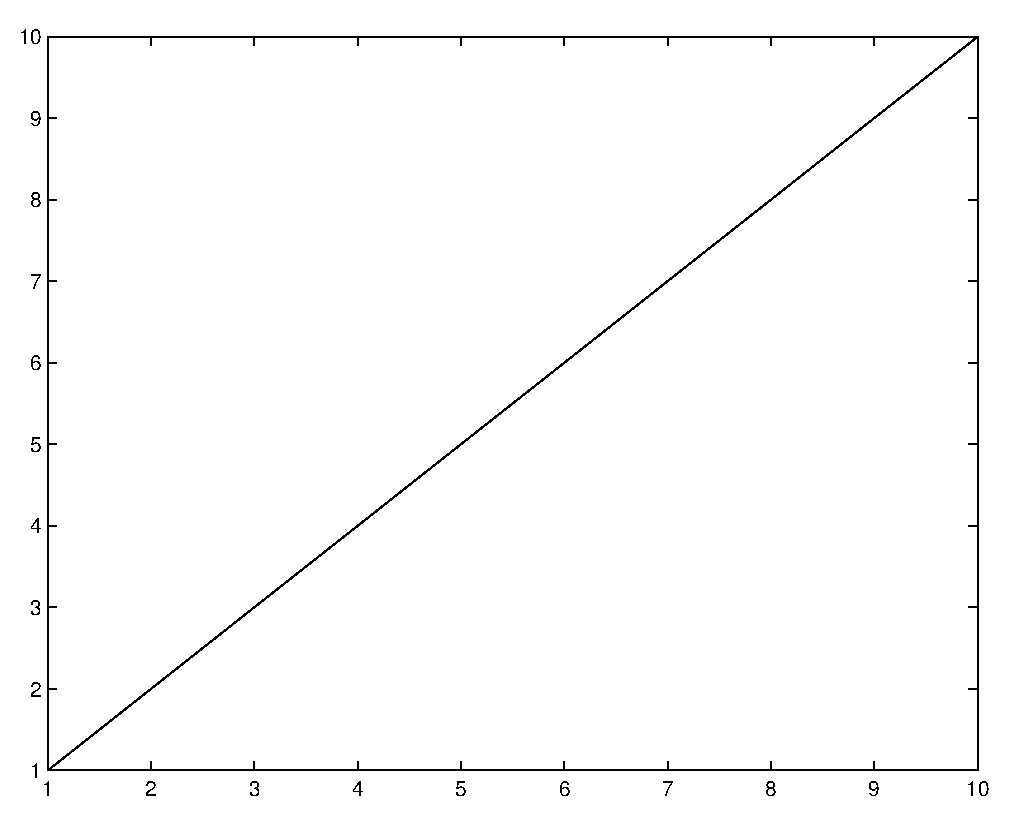
\includegraphics[scale=0.6]{epsFig.eps}
\end{center}

\section{Resultados}

Hicimos la elecci�n de direcciones de iluminaci�n con el procedimiento explicado en la parte de desarrollo y obtuvimos la siguiente matriz, que tiene el numero de condicion 15.0503:
\break
\\
$\begin{pmatrix} 0.15625000 & -0.59765625 & 0.78637964 \\ -0.11718750 & -0.57421875 & 0.81027151 \\ 0.03515625 & -0.44140625 & 0.89661840 \end{pmatrix}$
\break
\\
y la siguiente matriz que tiene el m�ximo numero de condici�n, 407,581:
\break
\\
$\begin{pmatrix} -0.03906250 & -0.56250000 & 0.82587400\\ -0.04296875 & -0.56250000 & 0.82567998\\ -0.04687500& -0.56250000 & 0.82546743 \end{pmatrix}$
\break
\\
Luego generamos los campos de las normales y obtuvimos los siguientes resultados:


\begin{center}
   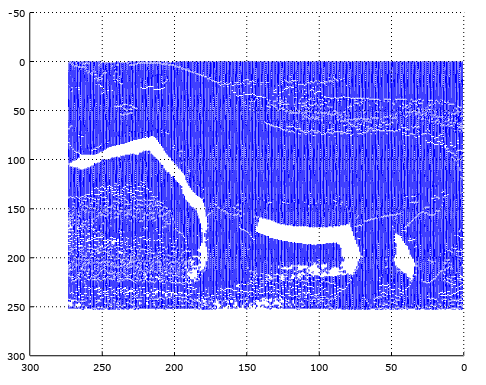
\includegraphics[scale=0.6]{caballoMax.png}
   \label{Fig. 1}
\end{center}

\begin{center}
   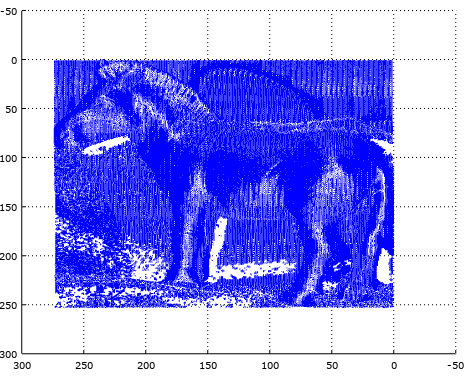
\includegraphics[scale=0.6]{caballoMin.png}
   \label{Fig. 2}
\end{center}

El siguiente grafico muestra los resultados que obtuvimos en e experimento donde comparamos las complejidades temporales del algoritmo de eliminacion de guass, la facotrizacion LU y Chelosky.

\begin{center}
   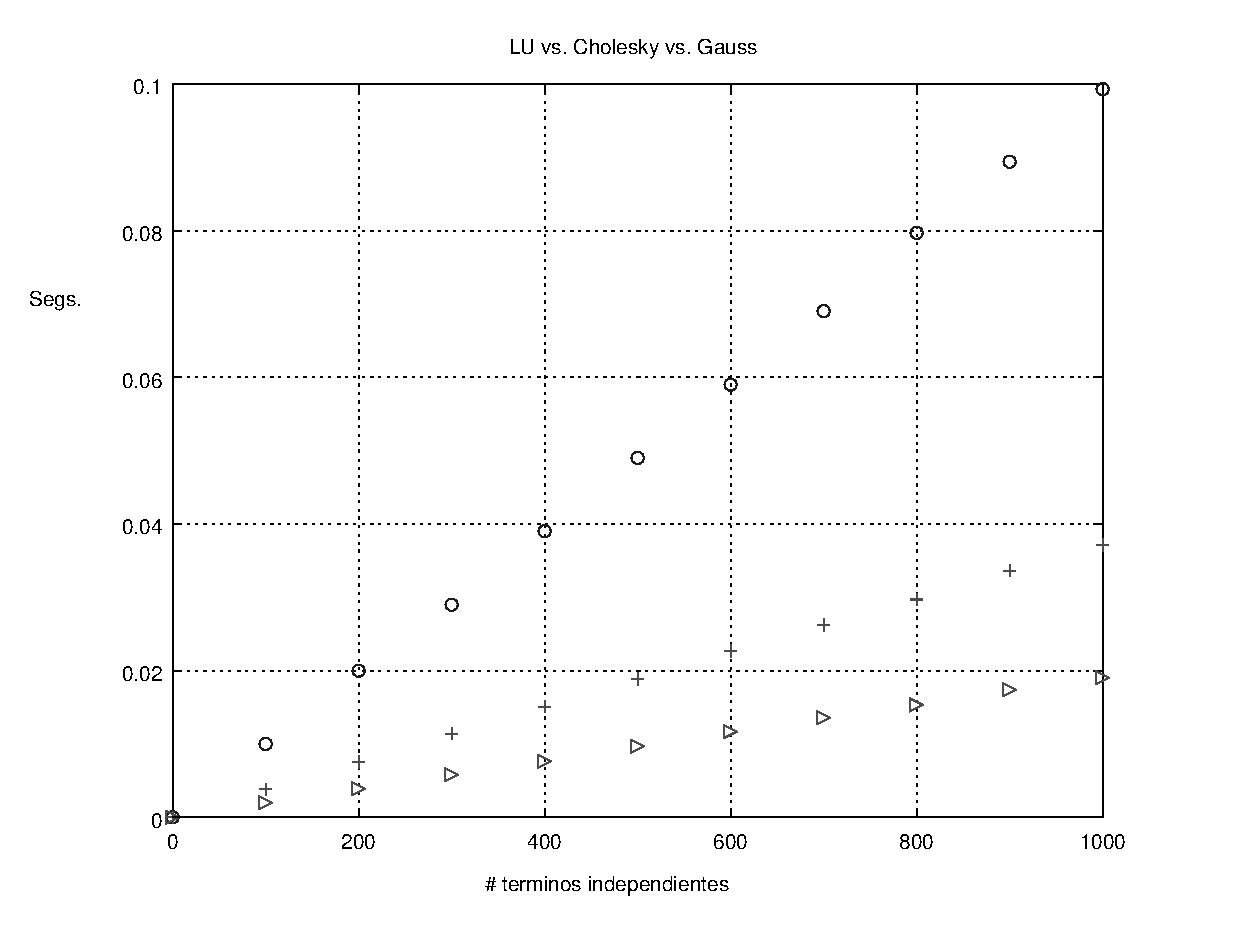
\includegraphics[scale=0.6]{LuCholeGauss.eps}
   \label{Fig. 3}
\end{center}

\begin{center}
   \includegraphics[scale=0.6]{graficochoto.png}
   \label{Fig. 3}
\end{center}


La imagen mate.6 tiene marcada con puntos de diferentes colores las siguientes vecindades: 0(negro), 2(rojo), 4(verde), 6(azul), 8(amarillo) y 10(cian).

\begin{center}
   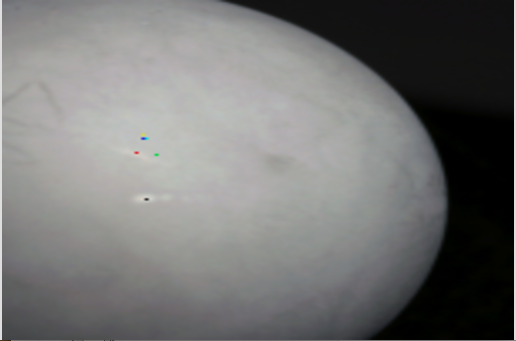
\includegraphics[scale=0.6]{ejemplo.png}
   \label{Fig. 4}
\end{center}


Los siguientes campos pertenecen al resultado de calibrar con vecindad cero y vecindad 6. 
\begin{center}
   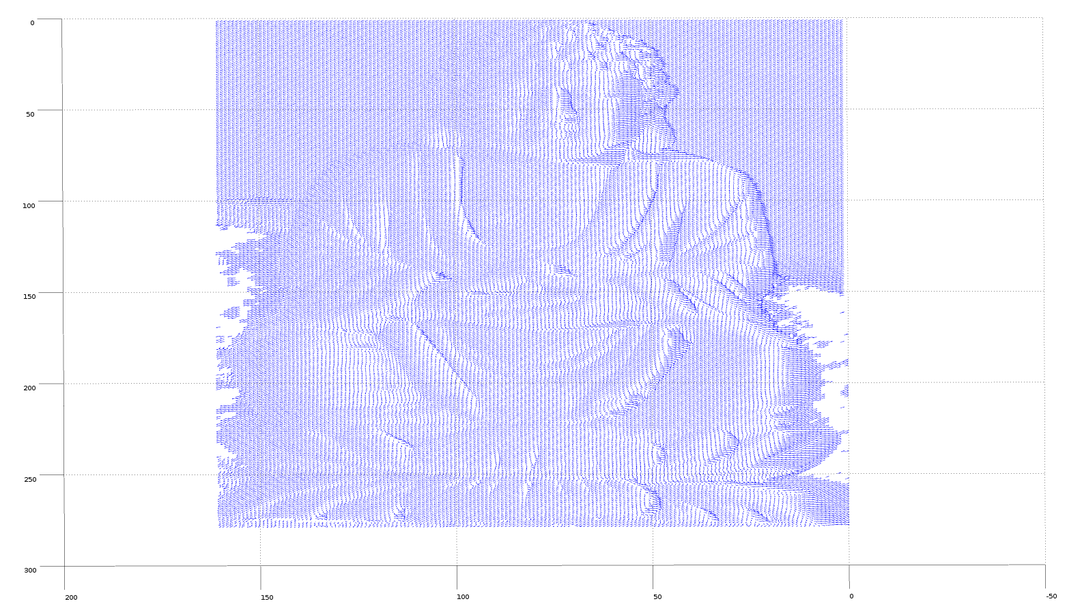
\includegraphics[scale=0.4]{buda_vecindad_0.png}
   \label{Fig. 4}
\end{center}

\begin{center}
   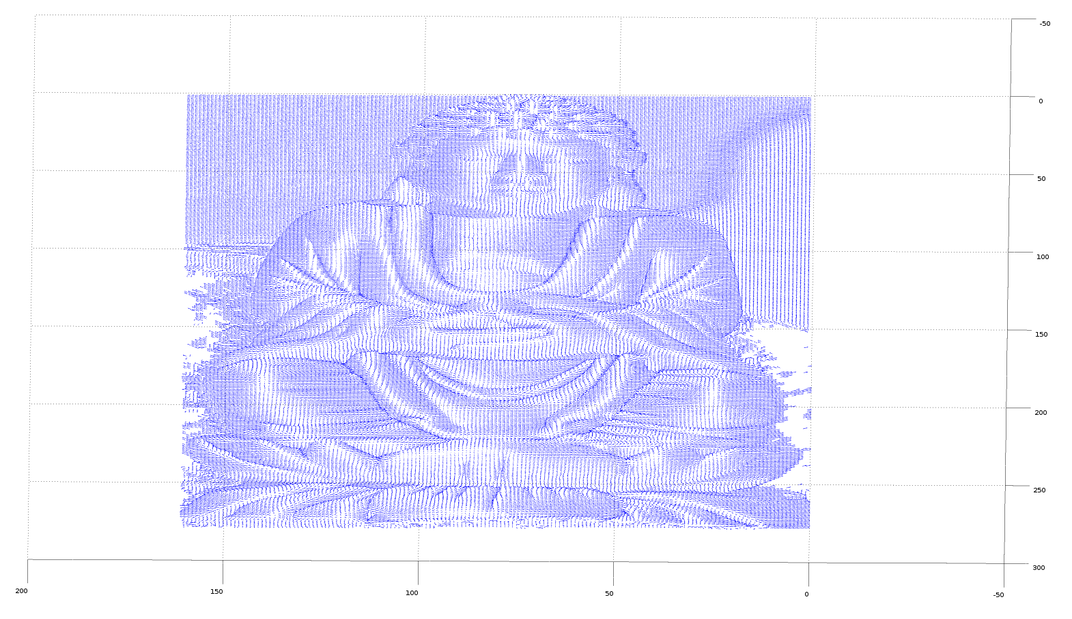
\includegraphics[scale=0.4]{buda_vecindades_6.png}
   \label{Fig. 5}
\end{center}






\indent Nuestra hip�tesis de que el numero de condici�n afecta directamente la estimaci�n de las normales se puede ver confirmada claramente en las im�gen del caballo. El campo de normales del caballo  en las figuras 1  esta estimado con la elecci�n de direcciones de iluminaci�n que causan que la matriz de la ecuaci�n 5 tanga el m�ximo numero de condici�n en comparaci�n a todas las otras posibles combinaciones de direcciones. En contraste la figura 2 utiliza la conbinaci�n de direcciones de illuminacion que generan la matriz con el mejor numero de condici�n. Esto se da porque un numero de condici�n alto implica que las direcciones de iluminaci�n est�n apuntando desde una posici�n muy similar lo cual es equivalente a tener una sola direccion para generar las normales y tambi�n las profundidades. \par


\section{Discusi\'on}

\subsection{Calibraci\'on}

\indent La imágen en la cual vimos la mayor diferencia es en Mate.6, d\'onde se observan esos factores de los que hablamos en el desarrollo, entre aquellos, las manchas de distinto color y la aureola de luz. P\'or ejemplo se ve el de vecindad 0 (p\'unto negro) bi\'en lejos de los demas, por lo claro de la mancha blanca. Las vecindades de 2 y 4 (rojo y verde) tambi\'en fueron corrompidos por el ruido, aunque llegaron un poco mas cerca. Luego a partir de los 6, 8 y 10 (az\'ul, amar\'illo y cian) se podria creer que llega a un lugar en donde por m\'as que agrandes el n\'umero de cantidad de vecindades no modificaria la posici\'on, tambi\'en vi\'endolo a simple vista se puede corroborar que es de d\'onde uno diria que proviene la luz.
Luego en el pr\'oximo experimento se observa que al modificar la cantidad de vecindades repercute fuertemente en la realizacion del resto del modelo, ya que con una mala direcci\'on de la luz se perdera el efecto 3D. \par

\subsection{Complejidades}

\indent Nuestra hipotesís, y a partir de lo que nos comentaron en las clases era que los algoritmos de eliminación gaussiana, factorización LU y Cholesky iban a tener un orden de complejidad cúbico y cuadrado, respectivamente, lo que al ver los resultados de las experimentaciones nos dice lo contrario. Las complejidades nos resultaron lineales, lo cual al pensarlo un momento se nos ocurrio que lo que puede estar pasando es debido a que la pendiente crece poco, a lo que deber\'iamos utilizar una cantidad may\'or de t\'erminos independientes. Esto \'ultimo no lo pudimos comprobar por falta de tiempo.  \par


\subsection{N\'umero de condici\'on}


\indent Nuestra hipótesis de que el n\'umero de condici\'on afecta directamente la estimaci\'on de las normales se puede ver confirmada claramente en las im\'agen del caballo. El campo de normales del caballo  en las figuras 1  esta estimado con la elección de direcciones de iluminaci\'on que causan que la matriz de la ecuaci\'on 5 tenga el m\'aximo n\'umero de condici\'on en comparaci\'on a todas las otras posibles combinaciones de direcciones. En contraste la figura 2 utiliza la conbinaci\'on de direcciones de iluminaci\'on que generan la matriz con el mejor n\'umero de condici\'on. Esto se da porque un n\'umero de condici\'on alto implica que las direcciones de iluminación est\'an apuntando desde una posici\'on muy similar lo cual es equivalente a tener una sola direcci\'on para generar las normales y tambi\'en las profundidades. \par

\subsection{RGB}

\indent La visi\'on humana tiende a diferenciar m\'as escalas de verde lo cual hace que al hacer un promedio ponderado para el color verde se obtengan mejores resultados. Esto lo tomamos en cuenta al momento de promediar los colores de los pixeles para buscar la direcci\'on proveniente de la luz. Al no poder encontrar una gran diferencia, decidimos utilizarlo.
(lo cuales no pudimos verlos en las imagenes que probamos)

//¿Como afectan la estimacion de las profundidades el calculo de las normales?


//¿Que metodos de solucion de los sistemas lineales arrojan mejores calculos de profundidades?

Aca escribimos las conclusiones.
¿Como afecta la calibracion del sistema en el resto de las etapas?
La calibracion es la parte inicial y fundamental para la resolucion de la reconstruccion 3D, ya que en ella obtenemos las direcciones de fuente de luz que afectara directamente al resultado, independientemente de que tan bueno sea el algoritmo para resolver sistemas lineales o estimar valores.

¿Como impacta la eleccion de las 3 direcciones de iluminacion para el calculo de las normales?
la eleccion de las direcciones de iluminacion afectara directamente a las normales ya que se aproximan apartir de ellas y si la matriz esta mal condicionada dara resultados no muy buenos.

\section{Conclusiones}

Aca escribimos las conclusiones.

\section{Ap\'endices}

Aca escribimos el apendices.

\section{Referencias}

1-Numerical Analysis - 9th Edition - (Burden and Faires)

\end{document}
